%!TEX TS-program = xelatex
%!TEX encoding = UTF-8 Unicode
%!TEX root = 2020-GS-ARTICLE.tex
%-------------------------------------------------------------------------------
%-------------------------------------------------------------------------------
%	PACKAGES AND OTHER DOCUMENT CONFIGURATIONS
%-------------------------------------------------------------------------------
%-------------------------------------------------------------------------------
\documentclass[
	a4paper,
	twocolumn
	]{article}
%--------------------------------------------------------------- GENERAL SETUP -
\usepackage[T1]{fontenc}
\usepackage[italian]{babel}
\usepackage{
  graphicx,
  dblfloatfix
}
\usepackage{graphicx}
\usepackage{epstopdf}
\epstopdfsetup{update}
\usepackage[usenames]{color}
\usepackage{amssymb}
\usepackage{hyperref} % For hyperlinks in the PDF
%---------------------------------------------------------------- STYLE GS2020 -
%-------------------------------------------------------------------------------
%-------------------------------------------------------------------------------
%	CUSTOM PACKAGES AND OTHER DOCUMENT CONFIGURATIONS
%-------------------------------------------------------------------------------
%-------------------------------------------------------------------------------
\usepackage{Alegreya}
\linespread{1.05}
\usepackage{
	fontspec,
	xltxtra,
	xunicode
	}

\usepackage{
	xfrac,
	unicode-math
	}

\defaultfontfeatures{Mapping=tex-text}
\setmonofont[
	Scale=MatchLowercase
	]{Andale Mono}
\setmathfont[
	Scale=MatchLowercase,
	Scale=1
	]{Libertinus Math}

\usepackage{microtype}
\usepackage[
	top=20mm,
	bottom=25mm,
	textwidth=17.2cm,
	columnsep=0.8cm
	]{geometry}
\usepackage[
	hang,
	small,
	labelfont=bf,
	up,
	textfont=it,
	up
	]{caption}
\usepackage{paralist} % For compact item lists
\usepackage{etoolbox} % Some tools: used for quote environment
\AtBeginEnvironment{quote}{\small}
\usepackage{titling} % Customizing the title section
\usepackage{booktabs} % Horizontal rules in tables
\usepackage{enumitem} % Customized lists
\setlist[itemize]{noitemsep} % Make itemize lists more compact
\usepackage{abstract} % Allows abstract customization
\renewcommand{\abstractnamefont}{\normalfont\bfseries} % Set the "Abstract" text to bold
\renewcommand{\abstracttextfont}{\normalfont\small\itshape} % Set the abstract itself to small italic text
\usepackage{titlesec} % Allows customization of titles
\renewcommand\thesection{\Roman{section}} % Roman numerals for the sections
\renewcommand\thesubsection{\Roman{subsection}} % roman numerals for subsections
\titleformat{\section}[block]{\large\centering}{\thesection.}{1em}{} % Change the look of the section titles
\titleformat{\subsection}[block]{\large}{\thesubsection.}{1em}{} % Change the look of the section titles
%-------------------------------------------------------------------------------
%-------------------------------------------------------------------------------
%	TITLE SECTION
%-------------------------------------------------------------------------------
%-------------------------------------------------------------------------------
\setlength{\droptitle}{-4\baselineskip} % Move the title up
\pretitle{\begin{center}\huge\bfseries} % Article title formatting
\posttitle{\end{center}} % Article title closing formatting
\title{Superstereo Synth \\ \large{\emph{Relazione STALPM}}} % Article title
\author{%
\textsc{Giuseppe Messineo}\\%[1ex]%
\normalsize Conservatorio G. Nicolini Piacenza \\ % Your institution
\normalsize giuseppe.messineo@conservatorio.piacenza.it % Your email address
%\and % Uncomment if 2 authors are required, duplicate these 4 lines if more
%\textsc{Wikio Orgopedio}\\%[1ex]%
%\normalsize Conservatorio S. Cecilia di Roma \\ % Your institution
%\normalsize wikio @ orgopedio.com % Your email address
}
\date{} % Leave empty to omit a date

\usepackage{fancyhdr} % Headers and footers
\pagestyle{fancy} % All pages have headers and footers
\fancyhead{} % Blank out the default header
\fancyfoot{} % Blank out the default footer
\fancyhead[C]{\small STALPM 1 • Relazione} % Custom header text
\fancyfoot[RO,LE]{\small \today~ • w: \input{includes/words.txt} • c: \input{includes/char.txt} • p:~\thepage} % Custom footer text
%-------------------------------------------------------------------------------
%-------------------------------------------------------------------------------
%	LISTINGS
%-------------------------------------------------------------------------------
%-------------------------------------------------------------------------------
\usepackage{listings}
% lstlistings setup
\definecolor{yobg}{rgb}{0.9,0.9,1}
\definecolor{yotxt}{rgb}{0.01,0.01,0.52} % a dark blue.
\definecolor{mylstbg}{rgb}{0.98,0.98,0.98} % a really pale grey.
\definecolor{mylstcmt}{rgb}{0.01,0.52,0.01} % a dark green.
\definecolor{mylstdoc}{rgb}{0.80,0.30,0.80} % a medium pink.

\lstset{%
  aboveskip=10pt,
	belowskip=5pt,
  language=C++,
  numbers=none,%left,%none,
  tabsize=4,
  %frame=single,
  breaklines=true,
  numberstyle=\tiny\ttfamily,
  backgroundcolor=\color{mylstbg},
  basicstyle=\footnotesize\ttfamily,
  commentstyle=\slshape\color{mylstcmt}, %\itshape,
  %frameround=tttt,
  columns=flexible, %fixed,
  showstringspaces=false,
  emptylines=2,
  inputencoding=utf8,
  extendedchars=true,
  literate=	{á}{{\'a}}1
			{à}{{\`a}}1
			{ä}{{\"a}}1
			{â}{{\^a}}1
			{é}{{\'e}}1
			{è}{{\`e}}1
			{ë}{{\"e}}1
			{ê}{{\^e}}1
			{ï}{{\"i}}1
			{î}{{\^i}}1
			{ö}{{\"o}}1
			{ô}{{\^o}}1
			{è}{{\`e}}1
			{ù}{{\`u}}1
			{û}{{\^u}}1
			{ç}{{\c{c}}}1
			{Ç}{{\c{C}}}1,
  emph={component, declare, environment, import, library, process},
  emph={[2]ffunction, fconstant, fvariable},
  emph={[3]button, checkbox, vslider, hslider, nentry, vgroup, hgroup, tgroup, vbargraph, hbargraph, attach},
  emphstyle=\color{yotxt}, %\underline, %\bfseries,
  morecomment=[s][\color{mylstdoc}]{<mdoc>}{</mdoc>},
  rulecolor=\color{black}
}

%-------------------------------------------------------------------- ABSTRACT -
\renewcommand{\maketitlehookd}{%
\begin{abstract}
\noindent\input{includes/abstract.txt}
\end{abstract}
}
%-------------------------------------------------------------------------------
%-------------------------------------------------------------------------------
%	BEGIN DOCUMENT
%-------------------------------------------------------------------------------
%-------------------------------------------------------------------------------
\begin{document}
\maketitle
\thispagestyle{empty}
%-------------------------------------------------------------------------------
%-------------------------------------------------------------------------------
\section*{INTRODUZIONE}
Partendo dal presupposto che la finalità del corso di STALPM 1 fosse quella
di costruire un oggetto multimimediale indirizzato al web e che quindi se ne
potesse usufruire anche in modo "non-locale", si è ragionato fin dalle prime
lezioni sulla tipologia d'oggetto da realizzare. Abbiamo quindi effettuato
un veloce brainstorming sicchè la realizzazione dell'oggetto multimediale
potesse sia portarci ad una finalità pratica, cioè quella di potere utilizzare
esso come un nostro strumento di composizione, sia di apprendimento dei concetti
basilari del mondo della programmazione (a noi sconosciuto o quasi fino a quel
momento) e non solo. Il frutto dei nostri ragionamenti è stato quello di realizzare un synth,
inizialmente con l'idea di basarci su di un modello fisico presistente, poi quella di
realizzarne uno con una struttura tutta sua, con specifici moduli e percorsi del segnale
totalmente nuovi, rispetto a quelli che erano i nostri pensieri al momento della decisione.
Per la realizzazione dello "Superstereo Synth" si è utilizzato Faust \cite{faust}
che utilizza un linguaggio di programmazione di tipo algebrico e dotato di IDE (interfaccia grafica), che
ha reso molto più fluido il nostro lavoro. Faust genera un codice c++, ed è quindi in grado
di essere multi-piattaforma, perfetto dunque per il nostro utilizzo. L'idea principale per
la construzione del nostro synth si è basata principalmente su un modulo di generazione sonora, un filtro e
un controllo d'ampiezza in uscita, per poi evolversi in qualcosa di più complesso \ref{superstereosynth} che verrà spiegata passo dopo passo nel paragrafo che segue. Il tutto è stato reso disponibile online \cite{heroku} grazie
a Heroku tramite Wasm (WebAssembly), linguaggio di basso livello che permette di far girare sul web applicazioni in maniera molto efficente.

\begin{figure}[h]
\begin{center}
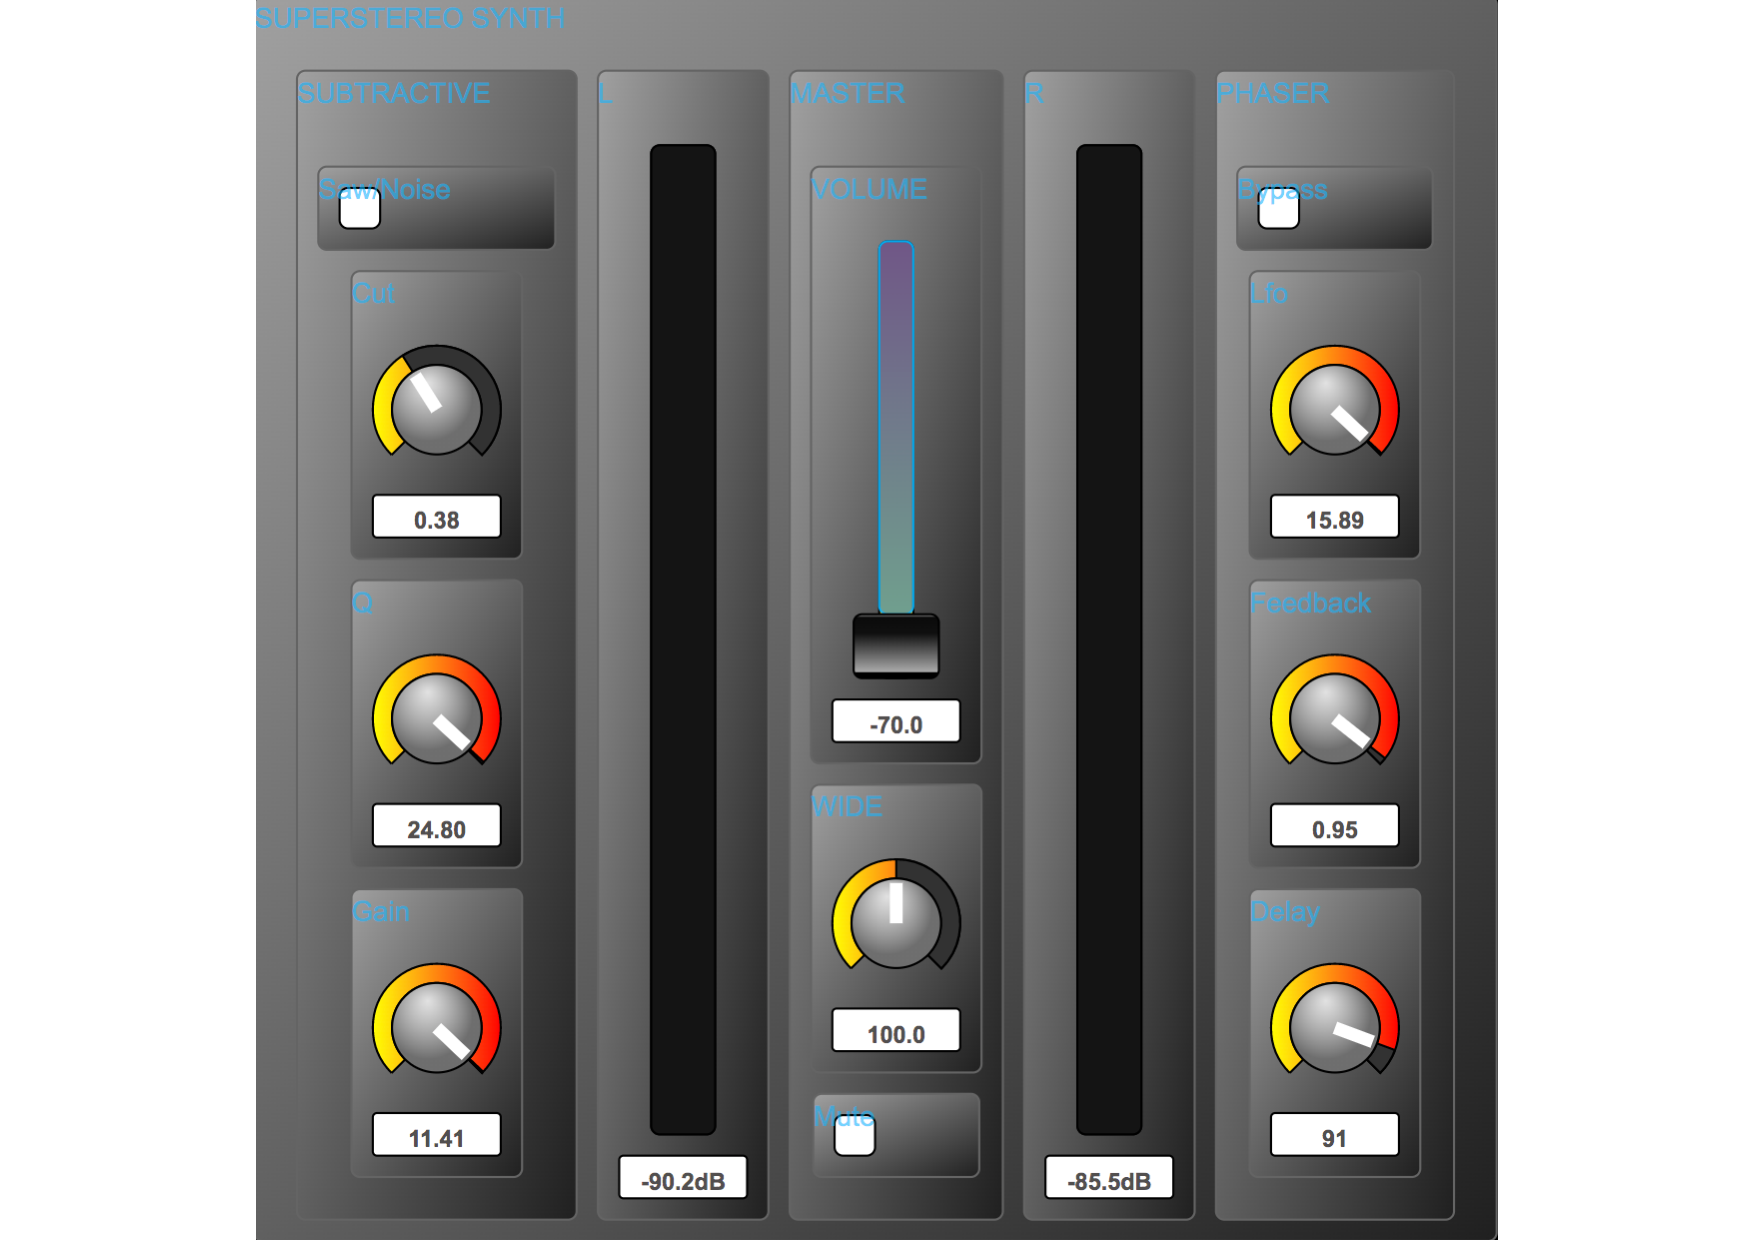
\includegraphics[width=.47\textwidth]{img/Superstereosynth}
\caption{\textbf{Superstereosynth}. Interfaccia grafica completa.}
\label{superstereosynth}
\end{center}
\end{figure}

%-------------------------------------------------------------------------------
\subsubsection*{DESCRIZIONE DEL CODICE}
La parte iniziale del codice denominata “GUI” contiene tutti i gruppi grafici dentro i quali abbiamo inserito i vari elementi –grafici appunto- del nostro strumento di sintesi quali knob, fader, pulsanti e meter.

%-----------------------------------------------------
%-------------------------larghezza massima del codice
\begin{lstlisting}
// GUI
main(x) = hgroup("[01] Superstereo Synth",x);
s_g(x) = main(vgroup("[01] SUBTRACTIVE",x));
m_g(x) = main(vgroup("[03] MASTER",x));
p_g(x) = main(vgroup("[05] PHASER",x));
lmeter(x) = main(attach(
	x,an.amp_follower(0.150,x) : ba.linear2db :
	vbargraph("[02] L [unit:dB]", -70,0)));
rmeter(x) = main(attach(
	x,an.amp_follower(0.150,x) : ba.linear2db :
	vbargraph("[04] R [unit:dB]", -70,0)));
meters = lmeter, rmeter;
\end{lstlisting}

Il modulo di sintesi sottrattiva chiamato “SUBTRACTIVE” contiene al suo interno un generatore di rumore bianco e uno di dente di sega con frequenza fissa (da noi indipendentemente scelta), swichabili tramite un apposito pulsante. Il tutto va dentro un filtro risonante “Ladder” basato sul modello di Robert Moog con relativi controlli di f cut e Q factor, ed in seguito ad un cotrollo di ampiezza.
Il modulo di sottrattiva è posto nella parte destra del synth.




%-----------------------------------------------------
%-------------------------larghezza massima del codice
\begin{lstlisting}
// SUBTRACTIVE
// Sawfreq Custom
sawfreq = 234;
generator = (no.noise *switch),
	(os.sawtooth(sawfreq)*(1-switch)) :> _;
switch = s_g(checkbox("[01] Saw/Noise")) : si.smoo;
gain = s_g(
	vslider("[04] Gain [style:knob]",-12,-96,+12,0.01))
	: ba.db2linear : si.smoo;
Q = s_g(
	vslider("[03] Q [style:knob]",5,0.7072,25,0.01));
fcut = s_g(
	vslider("[02] Cut [style:knob]",0.65,0,1,0.001)) :
	si.smoo;
subtractive = generator : ve.moogLadder(fcut,Q) :
	*(gain);
\end{lstlisting}


Di seguito troviamo un Phaser Stereo chiamato “PHASERSYNTH” (fig. \ref{phaser}),
costruito tramite una sequenza di N allpass, come dal modello di Curtis Roads su
“The Computer Music Tutorial” \cite{cr96cmt}, di cui il canale R dell'LFO agisce di fase opposta al
canale L. Il segnale verrà reso stereofonico tramite la tecnica dello
“Stereo Shuffling” (fig. \ref{stereoshuffler}), creando quindi due matrici SDM \cite{ab58} (somma-differenza) di
modo da avere un knob su cui poter controllare l'apertura stereofonica, agendo da solo segnale solo
monofonico (knob full sx) e superstereo (knob full dx). Lo “Superstereophaser”
(così chiamato, non solo lui ma anche lo stesso synth, citando il film “Ritorno al futuro”), avrà 3 tipi di controlli
tramite appositi knob:
\begin{compactitem}
\item LFO frequency
\item Feedback
\item Delay
\end{compactitem}



%-----------------------------------------------------
%-------------------------larghezza massima del codice
\begin{lstlisting}
// PHASER
lff = p_g(
	vslider("[02] Lfo [style:knob]",0.35, 0, 16, 0.001))
	: si.smoo;
fbk = p_g(
	vslider("[03] Feedback [style:knob]",
	        -0.689, -0.999, 0.999, 0.001) : si.smoo);
del = p_g(
	nentry("[04] Delay [style:knob]",1, 1, 100, 1));

lfo = os.osc(lff);

phaserLR(N,x,d,g,fb) = x <: l,r
with{
  allpassL(d,g) = (+ <: de.fdelay(
		(ma.SR/2),d),*(-g)) ~ *(g) : mem,_ : +;
  allpassR(d,g) = (+ <: de.fdelay(
		(ma.SR/2),d),*(g)) ~ *(-g) : mem,_ : +;
  apseqL(N,d,g) = seq(i,N,allpassL(d,g));
  apseqR(N,d,g) = seq(i,N,allpassR(d,g));

  l= _<: _, (+:apseqL(N,d,g))~*(fb):> _;
  r= _<: _, (+:apseqR(N,d,g))~*(-fb):> _;
};

// STEREO SHUFFLER
pot = m_g(
	vslider("[02] WIDE [style:knob]",100,0,200,0.1)) :
	/(100) : si.smoo;
somma = + : /(2);
diff = - : /(2);
sdm = somma,diff;
wide = _, * (sqrt(pot));
stereoshuffle= _,_ <: sdm : wide <: sdm;

superstereophaser = phaserLR(8,_,del,lfo,fbk) :
	stereoshuffle;
\end{lstlisting}
%-----------------------------------------------------
%-------------------------larghezza massima del codice

\begin{figure}[h]
\begin{center}
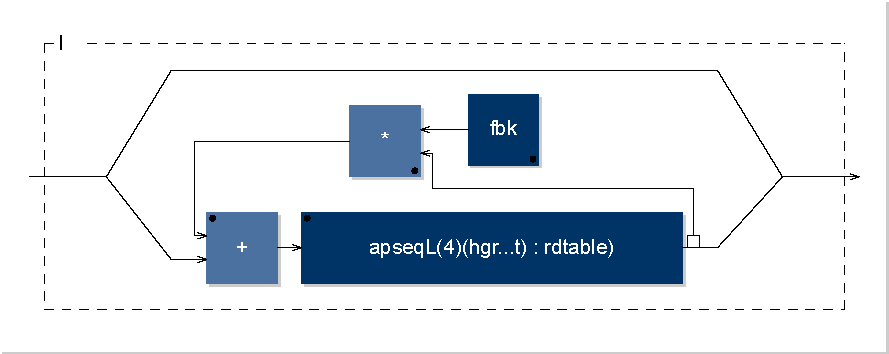
\includegraphics[width=.47\textwidth]{img/phaser}
\caption{\textbf{Phaser}. Realizzato con una serie di N allpass.}
\label{phaser}
\end{center}
\end{figure}

\begin{figure}[h]
\begin{center}
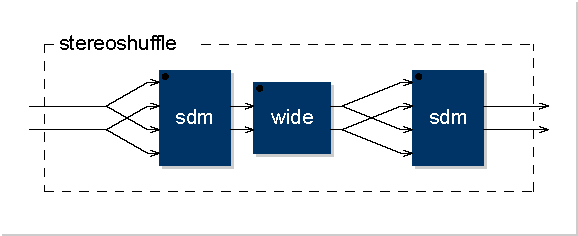
\includegraphics[width=.47\textwidth]{img/mid-side-shuffler}
\caption{\textbf{Stereo Shuffler}. Si possono notare nel diagramma a blocchi le due matrici SDM.}
\label{stereoshuffler}
\end{center}
\end{figure}

Lo “Superstereophaser” è posto sulla parte destra del synth e potrà essere bypassato tramite un apposito pulsante posto in cima alla sezione stessa.
Successivamente, il nostro segnale entrerà all’interno di un numero N di chopper o Hard Limiter (numero scelto diversamente da ogniuno di noi) che limiteranno il segnale in modo netto secondo una soglia prestabilita, seguiti da N filtri passa basso di diverso ordine (l'ordine dei filtri è stato scelto sempre in maniera indipendete da ogniuno di noi), in modo da rendere più “smooth” il segnale generato, attenuando le armoniche superiori generate dai chopper e mantenere quelle inferiori.

\begin{lstlisting}
// HARD LIMITER
chopper(a) = min(a) : max(-a);

hardlimiter = chopper(0.7) :
	fi.lowpass(12,15000): chopper(0.9) :
	fi.lowpass(8,2500): fi.lowpass6e(20000);
phchop = superstereophaser :
	hardlimiter, hardlimiter;
 \end{lstlisting}

Il tutto entrerà nella sezione chiamata “MASTER CONTROLS” nella quale avremo in ordine:
- Pulsante “MUTE”, che chiude il segnale alla fine della catena (pre-fader)
- Controllo del volume Master tramite un fader verticale con valori in scala logaritmica posto al centro del synth.
-Due Meters, sempre su scala logaritmica, posti al due lati della sezione Master.
La sezione Master si trova nella parte centrale del nostro Synth.

%-----------------------------------------------------
%-------------------------larghezza massima del codice
\begin{lstlisting}
// MASTER CONTROLS
mute = m_g(*(1-(checkbox("[04] Mute")))) : si.smoo;
volume = m_g(vslider("[02] VOLUME ",-6,-70,12,0.1)) :
   ba.db2linear : si.smoo;
bpc = p_g(checkbox("[01] Bypass"));
phaser = ba.bypass1to2(bpc,phchop);
mutes = mute,mute;
master = (*(volume), *(volume));
\end{lstlisting}

Di seguito la struttura generale del programma, sia in forma di codice che
rappresentata attraverso un diagramma a blocchi (fig. \ref{process}):

\begin{lstlisting}
process = subtractive : phaser : master : mutes : meters;
\end{lstlisting}

\begin{figure}[h]
\begin{center}
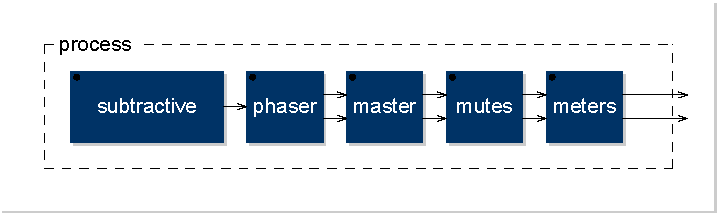
\includegraphics[width=.47\textwidth]{img/process}
\caption{\textbf{Process}. Diagramma a blocchi della struttura del synth.}
\label{process}
\end{center}
\end{figure}



% \newpage % USE NEWPAGE TO FORCE COLUMNN INTERRUPTION
%-------------------------------------------------------------------------------
%-------------------------------------------------------------------------------
\section*{CONCLUSIONI}
Devo ammettere che inizialmente l'idea di programmare da zero,
in questo caso un synth completo, mi intimoriva parecchio; in fin dei conti
però non è stato poi così complesso anzi, si è rivelato interessante e soprattutto
molto divertente. Mi è piaciuto come durante il corso, non ci venisse richiesto semplicemente
di "fare" una determinata cosa, ma venissimo guidati e indotti a ragionare su quali
fossero le possibili strade da percorrere. Non conoscevo Faust, ma ho imparato e sto imparando a
capirne le sue funzionalità e penso che sia un linguaggio abbastanza immediato e intuitivo,
grazie non solo alla sua documentazione, ma anche dalle righe di codice già disponibili che
possono essere studiate e analizzate con la possibilità di imparare molto da loro. Per quanto riguarda il synth
sono molto soddisfatto della sua resa sonora, a maggior ragione dopo le mie persanali modifiche; molto
probabilmente lo userò per delle mie personali composizioni, data la sua flessibilità
(posso ovviamente modificarlo, riprogrammando il codice). Credo che imparare e saper
governare la programmazione sia cosa più che fondamentale per un musicista del ventunesimo secolo.
A tal proposito, vorrei anche menzionare l'esperienza che nelle ultime lezioni abbiamo
affrontato con il linguaggio LaTeX \ref{latex} per la scrittura di questo paper, anch'essa molto utile a fronte
di una futura pubblicazione o anche semplicemente per la stesura
% (mi manca il termine)
della mia tesi di laurea. In sostanza, posso dire che aver seguito questo corso mi ha dato l'opportunità di
acquisire determinati valori aggiunti che non solo hanno arricchito il mio bagaglio di conoscenze,
ma hanno fatto accrescere in me la voglia smisurata di voler approfondire questo mondo.

\begin{figure}[h]
\begin{center}
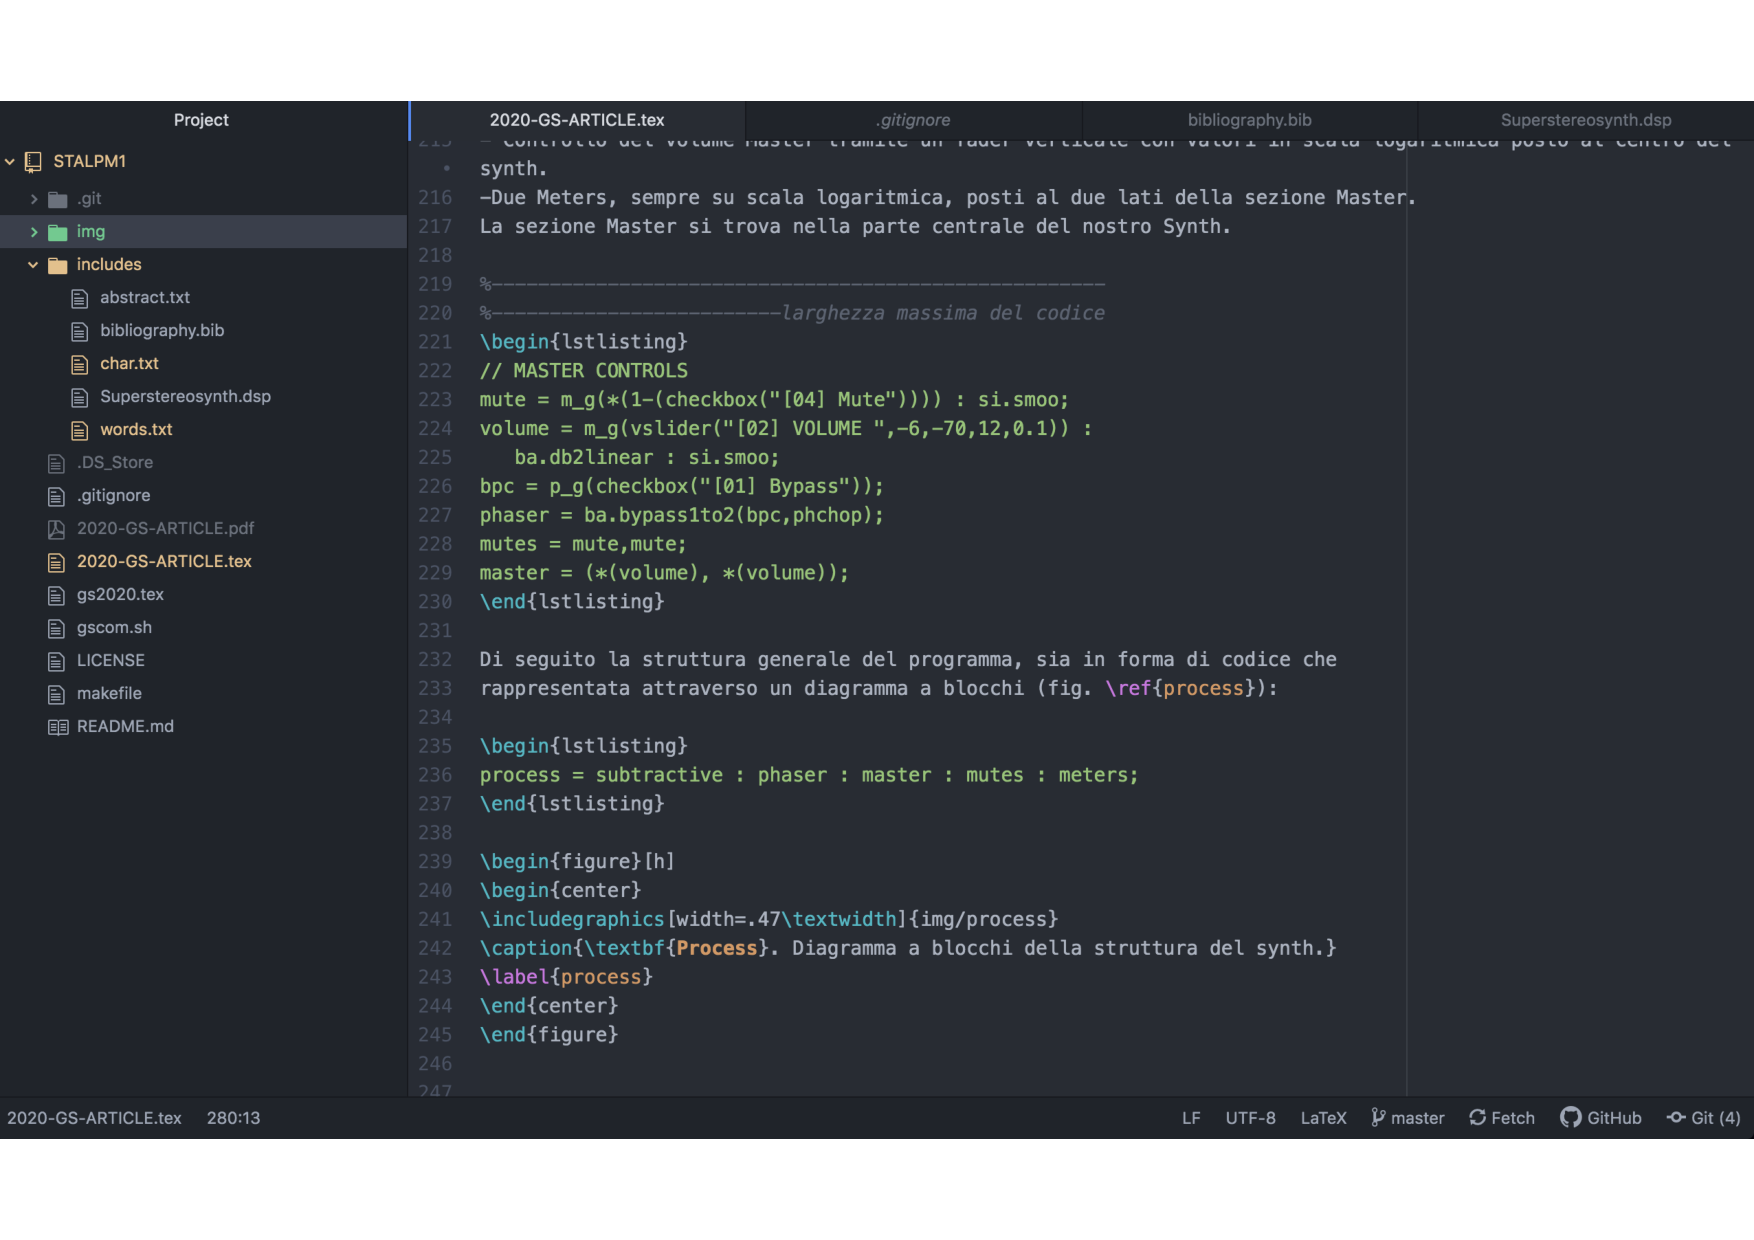
\includegraphics[width=.47\textwidth]{img/latex}
\caption{\textbf{Interfaccia di Atom}.Scrittura del paper con Atom e linguaggio LaTex.}
\label{latex}
\end{center}
\end{figure}
% \begin{quote}
% La musica non e` solo composizione. \\
% Non è artigianato, non è un mestiere. \\
% La musica è pensiero.\cite{nono85}.
% \end{quote}

% \begin{table}[htp]
% \begin{center}
% \begin{tabular}{ll}
% \textbf{Stages} & \textbf{Dur.} \\
% \hline
% \textbf{Omnidirectional Expositions} & 6 mo. \\
% Sound-shape analysis and visualizations & \\
% Sound-shape reproduction & \\
% Sound-shape database design & \\
% \hline
% \textbf{Micro-Rhythm of sound-shape} & 12 mo. \\
% Solo repertoire analysis & \\
% Sound-shape explosion in practising & \\
% From literature to shapes open-data & \\
% \hline
% \textbf{Rhythm of sound-shape interactions} & 12 mo. \\
% Multiple sources multiple shapes & \\
% Relationship and complexity perception & \\
% \hline
% \textbf{Sound-shape in musical composition} & 12 mo. \\
% AI: unleashed writing opportunities & \\
% AI: can you listen the time? & \\
% \hline
% \textbf{Final documentation} & 6 mo. \\
% \end{tabular}
% \label{timesheet}
% \caption{Thinking Tetrahedral Today stages}
% \end{center}
% \end{table}%


\vfill\null

\raggedright
\bibliographystyle{plain}
\bibliography{includes/bibliography.bib}

\end{document}

%%%%%%%%%%%%%%%%%%%%%%%%%%%%%%%%%%%%%%%%%%%%%%%%%%%%%%%%%%%%%%%%%%%%%%%%%%%%%%%%
% 2020 GIUSEPPE SILVI ARTICLE TEMPLATE BASED ON
%%%%%%%%%%%%%%%%%%%%%%%%%%%%%%%%%%%%%%%%%%%%%%%%%%%%%%%%%%%%%%%%%%%%%%%%%%%%%%%%
% Journal Article
% LaTeX Template
% Version 1.4 (15/5/16)
% This template has been downloaded from:
% http://www.LaTeXTemplates.com
% Original author:
% Frits Wenneker (http://www.howtotex.com) with extensive modifications by
% Vel (vel@LaTeXTemplates.com)
% License:
% CC BY-NC-SA 3.0 (http://creativecommons.org/licenses/by-nc-sa/3.0/)
%%%%%%%%%%%%%%%%%%%%%%%%%%%%%%%%%%%%%%%%%%%%%%%%%%%%%%%%%%%%%%%%%%%%%%%%%%%%%%%%
